\documentclass[letter, 12pt]{article}
\usepackage[T1]{fontenc}
\usepackage[spanish, mexico]{babel}
\usepackage[utf8]{inputenc}
\usepackage{booktabs} %Tablas.
\usepackage{float}
\usepackage{times}
\usepackage[margin=2.5cm]{geometry} %Margins.
\usepackage{amsmath,amssymb,amsthm} %Mathematics.
%\usepackage[none]{hyphenat} %No cortar las palabras.
\usepackage{setspace} %Espacios entre líneas.
\usepackage{graphicx} %Imágenes.
\usepackage{subfigure} %Varias imágenes dentro de una figura.
\usepackage{wrapfig} %Envolver imágenes con texto.
\usepackage{multicol} %Columnas.
\usepackage{multirow} %Unir celdas en tablas.
%\usepackage[hidelinks]{hyperref}

\title{Proyecto Personal Finanzas Computaciónales}
\author{Marina Morales }
\date{May 2022}

\begin{document}
\begin{titlepage}
    \begin{figure}[htbp]
        \centering
        \subfigure{\includegraphics[width=0.20\textwidth]{unam.png}  }\hspace{7cm}
        \subfigure{\includegraphics[width=0.20\textwidth]{fi.jpg}  }\vspace{0.5cm}
    \end{figure}
     \centering
    	{\scshape\LARGE Universidad Nacional Autónoma de México.\\Facultad de Ingeniería. \par}
    	\vspace{1cm}
    	{\huge \scshape Finanzas Computacionales\par}
    	\vspace{2cm}
    	{\bfseries \Large\textit{Proyecto grupal} \par}
    	\vspace{2cm}
    	{\Large Morales Luz Marina\\ \par}
    	{\Large Trejo Aldair\\ \par}
    	{\Large Selim Eduardo\\ \par}
    	\vfill
    	Profesor: Luis Vicente Montiel Cendejas.\\

    	\vfill

    	{\large Mayo 11, 2022.\\\par}
\end{titlepage}

{\large{\tableofcontents}} % Índice de contenidos
\cleardoublepage
\onehalfspacing
\section{Introducción.}




\section{Métricas}
\subsection{Promedios Moviles}
Dentro del análisis de series de tiempo, el promedio móvil nos permite mapear o rastrear las fluctuaciones teniendo en cuenta las tendencias más altas dentro de los datos.\\

Un promedio móvil es una técnica utilizada para suavizar los datos de series de tiempo para reducir el "ruido" en los datos e identificar más fácilmente patrones y tendencias.\\

En Moving Average, se calcula el promedio de diferentes partes (secciones) del conjunto de datos. Es decir, calcula el promedio general de los diversos subconjuntos dentro del conjunto de datos completo. Por esto, podemos entender la tendencia en los datos con respecto a diferentes escenarios o periodos temporales dentro del mismo conjunto de valores de datos que se aleatorizan por completo. Hay varios tipos de medias móviles, tales como:

- Promedio móvil simple

- Promedio móvil ponderado

- Media móvil exponencial


\subsection{Promedio Móvil Simple}

El promedio movil también es conocido como "rolling mean" y se calcula promediando los datos de la serie temporal dentro de k períodos de tiempo. Los promedios móviles se usan ampliamente en finanzas para determinar tendencias en el mercado y en ingeniería ambiental para evaluar estándares de calidad ambiental, como la concentración de contaminantes.\\

El pronóstico se obtiene calculando el promedio de los datos históricos considerados, es decir, pronostica con base al promedio de los períodos que se hayan considerado que se denominan orden del pronóstico. Dónde:

$$ F_{t}=\frac{C_{t}+C_{t-1}+...C_{t-9}}{n}$$\\

$F_{t}$= Pronóstico para el siguiente periodo.

$D_{t-i}$= Precios de cierre reales en los periodos pasados, (para i = 1… 10)

n = Numero de periodos para medir (en este caso utilizaremos n=10)

\subsection{Promedio Móvil Ponderado}

En el método de promedio móvil ponderado, hacemos uso de pesos para tener información sobre las fluctuaciones en los valores de los datos.\\

Aquí, se otorga un peso (valor) mayor a los datos que sean más recientes en la serie y un valor  más pequeño a los datos que son menos frecuente o son más antigüos en los valores de la serie.\\

Para calcular el promedio móvil ponderado (WMA), multiplicamos cada punto de datos con sus pesos correspondientes y finalmente calculamos la suma de los resultados.\\

Cuando se presenta una tendencia o un patrón localizable, pueden utilizarse ponderaciones para dar más énfasis a los valores recientes. Esta práctica permite que las técnicas de pronóstico respondan más rápido a los cambios,
puesto que puede darse mayor peso a los periodos más recientes. La elección de las ponderaciones es un tanto arbitraria porque no existe una fórmula establecida para determinarlas.\\

El promedio móvil ponderado utilizado en este caso se expresa como:

$$F_{t}=\frac{(10)C_{t}+(9)C_{t-1}+...C_{t-9}}{n+(n-1)+..+1} $$

$F_{t}$= Pronóstico para el siguiente periodo.

$D_{t-i}$= Precios de cierre reales en los periodos pasados, (para i = 1… 10)

n = Numero de periodos para medir (en este caso utilizaremos n=10)

\subsection{Stochastic K}

El oscilador estocástico es un indicador de momentum que se utiliza para indicar cambios de tendencia en el mercado de valores. Describe el precio actual en relación con los precios máximos y mínimos durante una serie de períodos de trading anteriores. \\

El oscilador estocástico fue desarrollado por el Dr. George Lane en la década de 1950 y se ha utilizado como indicador técnico para el comercio de acciones desde entonces. Su popularidad es atribuible a su relativa facilidad de interpretación y trayectoria de éxito. Este indicador a menudo se traza debajo de los gráficos de precios para ayudar a proporcionar señales visuales claras para las acciones comerciales.\\

El oscilador estocástico tiene 2 señales principales que funcionan para construir una señal comercial. Estas señales, denominadas señales rápidas y lentas. \\

El oscilador estocástico es un indicador de momentum que tiene en cuenta n valores previos durante una serie de tiempo. Esa es la definición técnica; en un lenguaje más sencillo, el oscilador estocástico utiliza el precio de los días de trading anteriores para describir qué tan cerca está el precio actual del rango (alto-bajo) durante esos días.\\

El oscilador estocástico en este caso se expresa como:

$$F_{t}=\frac{C_{t}-LL_{t-(n-1)}}{HH_{t-(n-1)}-LL_{t-(n-1)}}*100 $$

Donde:
LL y HH son el mínimo más bajo y el máximo más alto en los últimos t días, respectivamente.\\

\subsection{Larry William´s R}

El indicador Larry William´s es uno de los osciladores más populares entre aquellos que se utilizan para determinar si un mercado está sobrecomprado o sobrevendido. El indicador fue desarrollado por el famoso trader Larry Williams.\\




A continuación, hablaremos sobre cómo se calculan los valores del rango del porcentaje de Williams y luego pasaremos a analizar cómo usar en la práctica el indicador. Lo primero que debemos saber es que el indicador Williams R oscila en un rango de entre 0 y -100: \\

Para calcular la fórmula del indicador Williams, usamos el rango de porcentaje de Williams R usando la siguiente fórmula:


$$F_{t}=\frac{Nth High - Close}{Nth High - Nth Low} x (-100) $$ \\
Nth High: Precio más alto alcanzado durante el periodo analizado \\
Nth Low: Precio más bajo alcanzado durante el periodo analizado \\
Close: El precio final para el periodo analizado \\

Básicamente, esta fórmula se construye para cuantificar lo cerca que está el mercado de los límites externos de un rango reciente.

Un valor de $-100$ significa que el cierre actual es el mínimo más bajo de los últimos N periodos.

Un valor de 0 significa que el cierre actual es el más alto para los últimos N períodos.

Los valores intermedios muestran proporcionalmente dónde está el mercado entre estos dos extremos posibles.

\subsection{ A / D (Acumulación / Distribución Oscilador) }

El Indicador de Acumulación/Distribución es una herramienta de medición de volumen que evalúa la entrada y salida acumulada de dinero de un valor determinado. Mide el precio y el volumen del activo para determinar si se está acumulando o distribuyendo. \\

El indicador proporciona información sobre la fuerza de una tendencia. Por ejemplo, cuando el precio del activo está subiendo, pero el indicador A/D está bajando. Esto puede indicar que el volumen de acumulación, o compra, no es lo suficientemente fuerte como para soportar la subida del precio. Estas circunstancias podrían significar que una caída de precios será inminente a corto plazo.\\

El que desarrolló el indicador A/D fue el famoso trader y analista Marc Chaikin. Inicialmente se refirió a ella como la Línea de Flujo de Dinero Acumulativo. \\

En ese momento, solo pretendía que fuera una herramienta inteligente para la selección de valores. Los traders podían elegir una acción para comprar en función de la rapidez con la que creció el volumen y la cantidad de dinero que fluía hacia ella. A lo largo de los años, la línea de Acumulación/Distribución se ha convertido en un indicador popular en otros mercados, incluyendo el de Forex.

$$A / D =\frac{H_{t} - C_{t-1}}{H_{t} - L_{t}} $$
Es el precio de cierre: $C_{t-1}$ \\
Es el precio alto del tiempo t: $H_{t}$   \\
Es el precio bajo: $L_{t-1}$ \\


\section{Estadistica Descriptiva}

Se muestran los resultados del análisis descriptivo de las variables.

\subsection{Matriz de correlaciones}

     \begin{figure}[H]
    \centering
    \subfigure{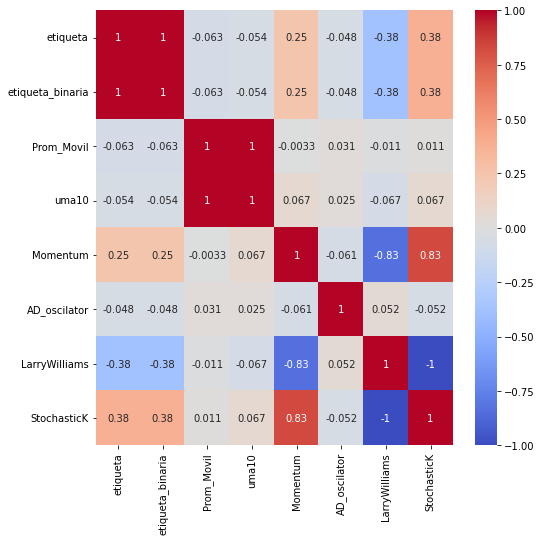
\includegraphics[width=0.60\textwidth]{matriz.png}}
    \end{figure}
Construimos una matriz de correlaciones,observamos que la métrica  Stochastic K tiene una correlación positiva  con la metricas Momentum, y una  correlación negativa con la metrica Larry William, con las démas metricas tiene poca correlación positiva.
\subsection{Box plot}

     \begin{figure}[H]
    \centering
    \subfigure{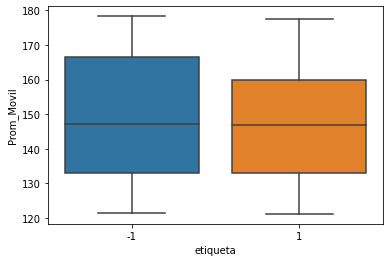
\includegraphics[width=0.60\textwidth]{prom_movil.png}}
    \end{figure}
En este gráfico visualizamos los resultados obtenidos al aplicar la metríca Promedio Moviles, y observamos que la media para la etiqueta -1 se enceuntra aproximadamente entre 145 a 148, el valor minimo se encuentra entre 122 a 124,el valor máximo es 176 a 178, con un rango intercuantil grande, es decir , tiene  variabilidad alta,  la asimetría de los datos es positiva, es decir la media es más grande que la mediana y la moda.

Para la etiqueta 1 y obtuvimos que la media para los -1 se enceuntra aproximadamente en 145 a 148, el valor minimo se encuentra entre 121 a 125,el valor máximo esta entre  175a 178, con un rango intercuantil grande.
    \begin{figure}[H]
    \centering
    \subfigure{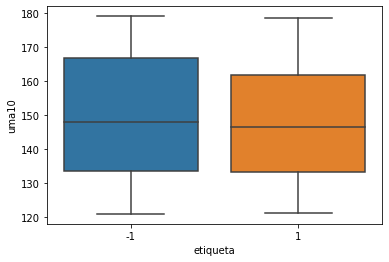
\includegraphics[width=0.60\textwidth]{uma10.png}}
    \end{figure}
En este grafico visualizamos los resultados obtenidos al aplicar la metríca Promedio Moviles, y obtuvimos que la media para los -1 se enceuntra aproximadamente en 145 a 148, el valor minimo se encuentra entre 121 a 125,el valor máximo esta entre  175a 178, con un rango intercuantil de  , la asimetría de los datos es positiva, es decir la media es más grande que la mediana y la moda.

Para la etiqueta 1 y obtuvimos que la media para los -1 se enceuntra aproximadamente en 145 a 148, el valor minimo se encuentra entre 121 a 125,el valor máximo esta entre  175a 178, con un rango intercuantil de  , la asimetría de los datos es positiva, es decir la media es más grande que la mediana y la moda.
     \begin{figure}[H]
    \centering
    \subfigure{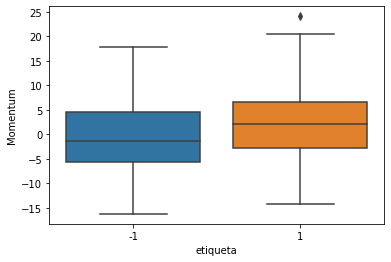
\includegraphics[width=0.60\textwidth]{momentum.png}}
    \end{figure}
En este grafico visualizamos los resultados obtenidos al aplicar la metríca Momentum, y obtuvimos que la media para los -1 se enceuntra aproximadamente en -3 a -1, el valor minimo se encuentra en -15,el valor máximo esta entre  16 a 18, con un rango intercuantil relativamente bajo  , la asimetría de los datos es positiva, es decir la media es más grande que la mediana y la moda.

Para la etiqueta 1 obtuvimos que la media se encuentra  aproximadamente entre -3 a -1, el valor minimo se encuentra en -15,el valor máximo esta entre  16 a 18, con un rango intercuantil relativamente bajo  , los datos son simetricos.
     \begin{figure}[H]
    \centering
    \subfigure{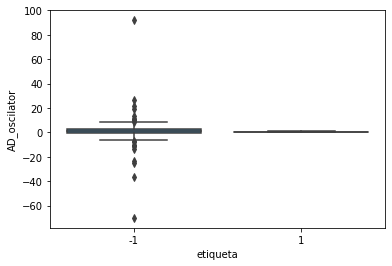
\includegraphics[width=0.60\textwidth]{ad_osci.png}}
    \end{figure}
En este grafico visualizamos los resultados obtenidos al aplicar la metríca ADOscilator, para la etiqueta -1 , y podemos decir que los datos estan concentrados, porque no se aprecia con  los cuantiles, tiene valores varios valores atipicos //

Para la etiqueta 1, los datos estan concentrados, es decir, no tiene mucha variabilidad, no encontramos datos atipicos.
     \begin{figure}[H]
    \centering
    \subfigure{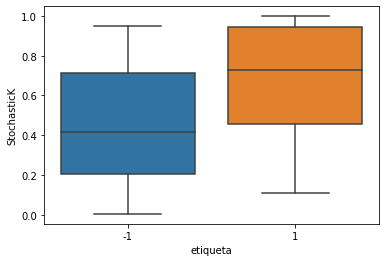
\includegraphics[width=0.60\textwidth]{osi_esto.png}}
    \end{figure}
Los resultados obtenidos al aplicar la metríca Stochastic K, para la etiqueta -1 se enceuntra aproximadamente en 0.4, el valor minimo se encuentra en 0,el valor máximo esta en .9, con un rango intercuantil de .9 ,la variabilidad es poca,  la asimetría de los datos es positiva, es decír, la media es más grande que la mediana y la moda.

Para la etiqueta 1, obtuvimos que la media esta en .7, el valor minimo se encuentra en .1, el valor máximo esta en 1, con un rango intercuantil de .9.
    \begin{figure}[H]
    \centering
    \subfigure{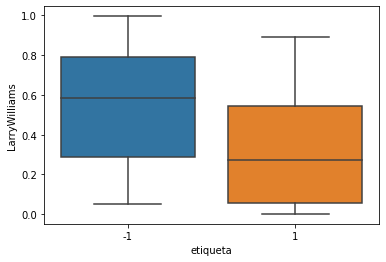
\includegraphics[width=0.60\textwidth]{larry_williams.png}}
    \end{figure}
En este grafico visualizamos los resultados obtenidos al aplicar la metríca Larry William, y obtuvimos que la media para la etiqueta -1 se encuentra en .6, el valor minimo se encuentra en .1 ,el valor máximo es 1, con un rango intercuantil de  .9.\\

Para la etiqueta 1 y obtuvimos que la media es .3, el valor minimo se encuentra en .1,el valor máximo esta en 1.

\subsection{Histogramas}



\begin{figure}[H]
    \centering
    \subfigure{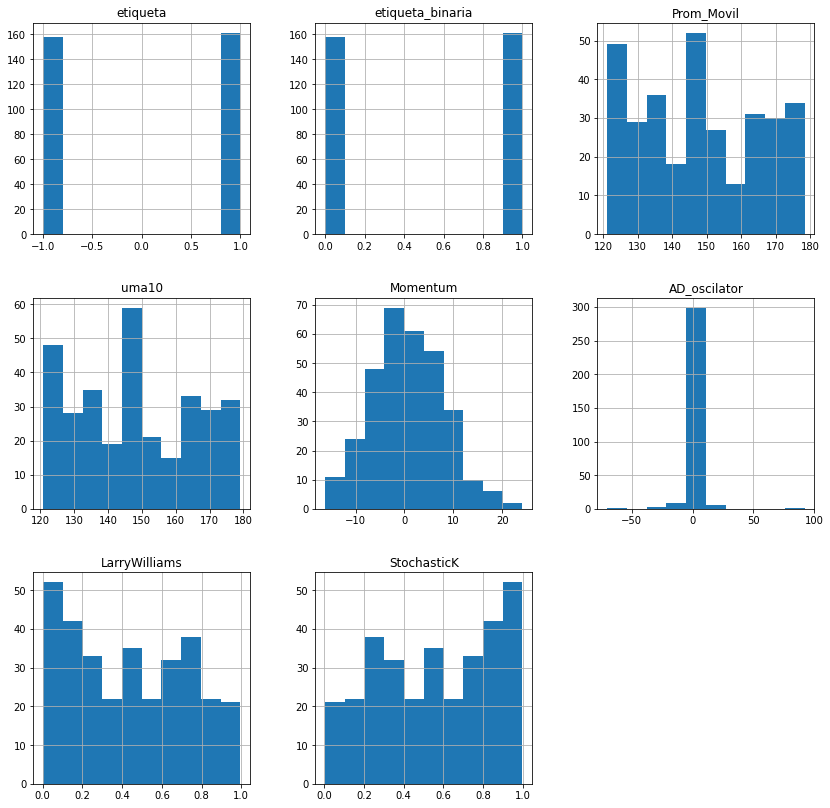
\includegraphics[width=0.8\textwidth]{histogramas.png}}
    \end{figure}

En este grafico visualisamos la distribución de las metricas y los indicadores, para el promedio movil vemos que la moda (el dato que más se repite) es 145 , despues es 125, no tenemos sospecha de una distribucón conocida, para el caso del indicador UMA vemos que la moda es 145, la forma de esta graficas es similar al de promedio movil, para el indicador Momentum encontramos que los datos estan un poco mas concentrados en la media, pero tiene una asimetria a la izquierda, el indicador A D Oscilador se centra e la media que esta en 0, la mayoría de los datos estan concentrados en la media,sin embargo, existen datos atipicos.
Para el indicador Larry William observamos que tiene una tendencia descendiente ,para el indicador Stochastic K tiene un comportamiento diferente, es decir, va en crecimiento  

\begin{thebibliography}{10} 

* Patel,Shah,Thakka,Kotecha(2014). Predicting stock market index using fusion of machine learning techniques. Expert Systems with Applications.ELSEVIER\\


* Patel,Shah,Thakka,Kotecha(2014). Predicting stock market index using fusion of machine learning techniques. Expert Systems with Applications.ELSEVIER\\


* Using the Stochastic Oscillator in Python for Algorithmic Trading: \\  https://www.alpharithms.com/stochastic-oscillator-in-python-483214/\\


* Calculate Weighted Moving Average in Python:\\ https://www.journaldev.com/50471/weighted-moving-average-in-python\\


\end{thebibliography}

\end{document}










\end{document}